\iffalse
\let\negmedspace\undefined
\let\negthickspace\undefined
\documentclass[journal,12pt,twocolumn]{IEEEtran}
\usepackage{cite}
\usepackage{amsmath,amssymb,amsfonts,amsthm}
\usepackage{algorithmic}
\usepackage{graphicx}
\usepackage{textcomp}
\usepackage{xcolor}
\usepackage{txfonts}
\usepackage{listings}
\usepackage{enumitem}
\usepackage{mathtools}
\usepackage{gensymb}
\usepackage{comment}
\usepackage[breaklinks=true]{hyperref}
\usepackage{tkz-euclide}
\usepackage{listings}
\usepackage{gvv}
\def\inputGnumericTable{}
\usepackage[latin1]{inputenc}
\usepackage{color}
\usepackage{array}
\usepackage{longtable}
\usepackage{calc}
\usepackage{multirow}
\usepackage{hhline}
\usepackage{ifthen}
\usepackage{lscape}

\newtheorem{theorem}{Theorem}[section]
\newtheorem{problem}{Problem}
\newtheorem{proposition}{Proposition}[section]
\newtheorem{lemma}{Lemma}[section]
\newtheorem{corollary}[theorem]{Corollary}
\newtheorem{example}{Example}[section]
\newtheorem{definition}[problem]{Definition}
\newcommand{\BEQA}{\begin{eqnarray}}
\newcommand{\EEQA}{\end{eqnarray}}
\newcommand{\define}{\stackrel{\triangle}{=}}
\theoremstyle{remark}
\newtheorem{rem}{Remark}
\begin{document}

\bibliographystyle{IEEEtran}
\vspace{3cm}

\title{NCERT Discrete - 10.5.3.20}
\author{EE23BTECH1205 - Avani Chouhan$^{*}$% <-this % stops a space
}
\maketitle
\newpage
\bigskip

\renewcommand{\thefigure}{\theenumi}
\renewcommand{\thetable}{\theenumi}

\vspace{3cm}
\textbf{Question : 10.5.3.20} 
The sum of some terms of G.P. is 315 whose first term and the common ratio are $5$ and $2$ , respectively. Find the last term and the number of terms.\\
\solution
\fi
\begin{table}
  \centering
  \begin{tabular}{|c|c|c|}
    \hline
    \textbf{Parameter} & \textbf{Value} & \textbf{Description} \\
    \hline
    $x(0)$ & $5$ & First term \\
    \hline
    $r$ & $2$ & Common ratio \\
    \hline
    $y(n)$ & $315$ & Sum of $n+1$ terms \\
    \hline
    $x(n)$ & ? & Last term\\
    \hline
\end{tabular}


  \caption{Input Parameters}
  \label{tab:10.5.3.20table1}
\end{table}
\begin{align}
x(n) = x(0)r^{n}u(n)
\label{eq:10.5.3.20eq}
\end{align}
From \eqref{eq:gpz}
\begin{align}
X(z) =\frac{5}{1-2z^{-1}} \quad \abs{z} > \abs{2}
\end{align}
By contour integration:
\begin{align}
y(n) &= x(0)\brak{\frac{r^{n+1}-1}{r-1}}u(n)\\
315 &= 5\brak{2^{n+1}- 1}  \\
\implies n &= 5
\end{align}
The number of terms is \(n + 1 = 6\)\\
From \eqref{eq:10.5.3.20eq}:
\begin{align}
x(5) &= 5\brak{2^{5}}\\
 &= 160 
\end{align}

\begin{figure}[H]
    \centering
    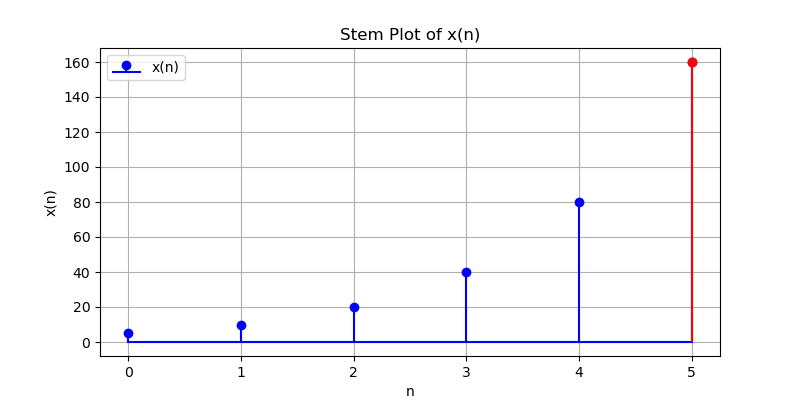
\includegraphics[width=\columnwidth]{ncert-maths/11/9/5/8/figs/plot1.png}
    \caption{Stem plot of x(n)}
    \label{fig:10.5.3.20fig1}
\end{figure}
\begin{figure}[H]
    \centering
    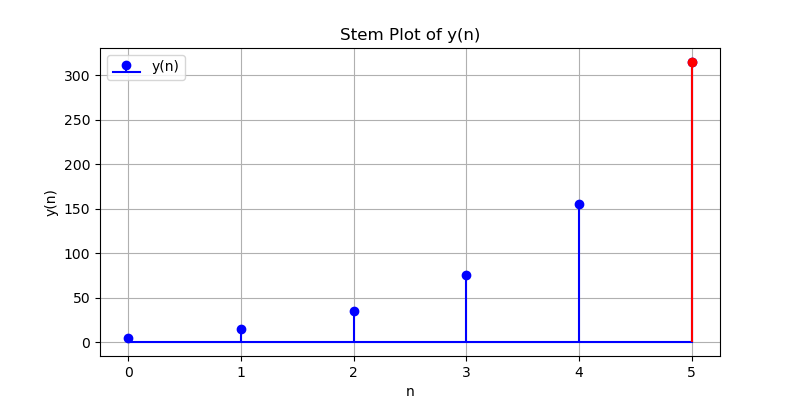
\includegraphics[width=\columnwidth]{ncert-maths/11/9/5/8/figs/plot2.png}
    \caption{Stem plot of y(n)}
    \label{fig:10.5.3.20fig2}
\end{figure}
%\end{document}
